% YZM5110 Research Project -- 5-minute introductory talk (19 Nov 2026 session).
% The instructor asked for a short talk that introduces the topic to classmates; the detailed account of what was
% tried and what worked is in the report (report/Ucuran_YZM5110_Research.pdf) and in the detailed deck (slides.pdf).
% Build:  python scripts/make_report_tables.py && python scripts/make_figures.py && cd slides && tectonic short_talk.tex
% Measured numbers are macros from ../report/generated/numbers.tex; published numbers are typed by hand and cited.
\documentclass[aspectratio=169,11pt]{beamer}
\usepackage[T1]{fontenc}
\usepackage{lmodern}
\usepackage{amsmath}
\usepackage{xcolor}
\usepackage{tikz}
\usetikzlibrary{positioning,arrows.meta,calc}
% generated by scripts/make_report_tables.py -- do not edit
\newcommand{\nQueries}{451}
\newcommand{\nPages}{500}
\newcommand{\nDup}{22}
\newcommand{\pubCard}{0.585}
\newcommand{\pubPaper}{0.544}
\newcommand{\fullB}{0.575}
\newcommand{\fullA}{0.391}
\newcommand{\fullBGE}{0.249}
\newcommand{\gapCardPts}{$-$0.94}
\newcommand{\pubBMtwentyfive}{0.368}
\newcommand{\pubBGE}{0.257}
\newcommand{\fullBnodup}{0.601}
\newcommand{\nDev}{226}
\newcommand{\devB}{0.580}
\newcommand{\devA}{0.400}
\newcommand{\devBGE}{0.235}
\newcommand{\devCkone}{0.534}
\newcommand{\devDkone}{0.526}
\newcommand{\devCksixty}{0.467}
\newcommand{\devDksixty}{0.422}
\newcommand{\devCw}{0.585}
\newcommand{\devDw}{0.580}
\newcommand{\devCwGainPts}{+0.47}
\newcommand{\nWgrid}{9}
\newcommand{\nKgrid}{10}
\newcommand{\nTest}{225}
\newcommand{\testA}{0.382}
\newcommand{\testACI}{[0.323, 0.441]}
\newcommand{\deltaA}{$-$0.188}
\newcommand{\deltaACI}{[$-$0.237, $-$0.142]}
\newcommand{\pHolmA}{$<$0.001}
\newcommand{\pA}{$<$0.001}
\newcommand{\wtlA}{10/144/71}
\newcommand{\testBGE}{0.262}
\newcommand{\testBGECI}{[0.209, 0.317]}
\newcommand{\deltaBGE}{$-$0.308}
\newcommand{\deltaBGECI}{[$-$0.364, $-$0.252]}
\newcommand{\pHolmBGE}{$<$0.001}
\newcommand{\pBGE}{$<$0.001}
\newcommand{\wtlBGE}{5/122/98}
\newcommand{\testB}{0.570}
\newcommand{\testBCI}{[0.510, 0.627]}
\newcommand{\testC}{0.516}
\newcommand{\testCCI}{[0.457, 0.574]}
\newcommand{\deltaC}{$-$0.054}
\newcommand{\deltaCCI}{[$-$0.076, $-$0.032]}
\newcommand{\pHolmC}{$<$0.001}
\newcommand{\pC}{$<$0.001}
\newcommand{\wtlC}{9/167/49}
\newcommand{\testD}{0.519}
\newcommand{\testDCI}{[0.460, 0.578]}
\newcommand{\deltaD}{$-$0.051}
\newcommand{\deltaDCI}{[$-$0.072, $-$0.030]}
\newcommand{\pHolmD}{$<$0.001}
\newcommand{\pD}{$<$0.001}
\newcommand{\wtlD}{4/171/50}
\newcommand{\testCw}{0.571}
\newcommand{\testCwCI}{[0.511, 0.629]}
\newcommand{\deltaCw}{+0.001}
\newcommand{\deltaCwCI}{[$-$0.002, +0.005]}
\newcommand{\pHolmCw}{1.000}
\newcommand{\pCw}{0.937}
\newcommand{\wtlCw}{2/220/3}
\newcommand{\testDw}{0.570}
\newcommand{\testDwCI}{[0.510, 0.627]}
\newcommand{\deltaDw}{+0.000}
\newcommand{\deltaDwCI}{[+0.000, +0.000]}
\newcommand{\pHolmDw}{1.000}
\newcommand{\pDw}{1.000}
\newcommand{\wtlDw}{0/225/0}
\newcommand{\deltaCvsD}{$-$0.003}
\newcommand{\deltaCvsDCI}{[$-$0.027, +0.021]}
\newcommand{\pCvsD}{0.844}
\newcommand{\wtlCvsD}{25/174/26}
\newcommand{\pCwvsDw}{0.937}
\newcommand{\nexact}{93}
\newcommand{\typeexactA}{0.617}
\newcommand{\typeexactB}{0.833}
\newcommand{\typeexactC}{0.774}
\newcommand{\typeexactD}{0.771}
\newcommand{\ngeneral}{115}
\newcommand{\typegeneralA}{0.231}
\newcommand{\typegeneralB}{0.391}
\newcommand{\typegeneralC}{0.345}
\newcommand{\typegeneralD}{0.343}
\newcommand{\nvisual}{17}
\newcommand{\typevisualA}{0.118}
\newcommand{\typevisualB}{0.339}
\newcommand{\typevisualC}{0.265}
\newcommand{\typevisualD}{0.331}
\newcommand{\nNoDup}{212}
\newcommand{\noDupB}{0.598}
\newcommand{\noDupC}{0.542}
\newcommand{\noDupDeltaC}{$-$0.056}
\newcommand{\noDupDeltaCw}{+0.001}
\newcommand{\peakGPU}{15.8}
\newcommand{\latB}{51.3}
\newcommand{\latA}{0.12}
\newcommand{\latBGE}{29.0}
\newcommand{\fusionOverhead}{0.13}
\newcommand{\idxB}{111.7}
\newcommand{\sizeB}{126}
\newcommand{\headallAnotB}{3}
\newcommand{\headallBnotA}{50}
\newcommand{\headexactAnotB}{0}
\newcommand{\headexactBnotA}{22}
\newcommand{\headgeneralAnotB}{3}
\newcommand{\headgeneralBnotA}{23}
\newcommand{\headvisualAnotB}{0}
\newcommand{\headvisualBnotA}{5}
\newcommand{\hitB}{147}
\newcommand{\hitA}{100}
\newcommand{\oracle}{150}
\newcommand{\bothMiss}{75}
\newcommand{\oracleNDCG}{0.588}
\newcommand{\oracleGainPts}{+1.8}
\newcommand{\oracleAbetter}{10}
\newcommand{\cWins}{9}
\newcommand{\cLosses}{49}
\newcommand{\cLossBMmissed}{42}
\newcommand{\cwChanged}{5}
\newcommand{\ovAhit}{0.73}
\newcommand{\ovAmiss}{0.18}
\newcommand{\ovZeroN}{75}
\newcommand{\ovZeroA}{0}
\newcommand{\ovZeroB}{23}
\newcommand{\ovOneN}{43}
\newcommand{\ovOneA}{91}
\newcommand{\ovOneB}{95}
\newcommand{\fullAcode}{0.402}
\newcommand{\devAcode}{0.399}
\newcommand{\testAcode}{0.405}
\newcommand{\deltaAcodeA}{+0.023}
\newcommand{\deltaAcodeACI}{[+0.004, +0.046]}
\newcommand{\pAcodeA}{0.027}
\newcommand{\wtlAcodeA}{14/206/5}
\newcommand{\typeexactAcode}{0.667}
\newcommand{\testCcode}{0.525}
\newcommand{\deltaCcode}{$-$0.045}
\newcommand{\deltaCcodeCI}{[$-$0.066, $-$0.024]}
\newcommand{\pHolmCcode}{$<$0.001}
\newcommand{\deltaCcodevsC}{+0.009}
\newcommand{\pCcodevsC}{0.091}
\newcommand{\alphaCcc}{1.0}
\newcommand{\alphaDcc}{1.0}
\newcommand{\devBestBelowOneCcc}{0.575}
\newcommand{\devBestBelowOneAlphaCcc}{0.95}
\newcommand{\devBestBelowOneDcc}{0.576}
\newcommand{\devBestBelowOneAlphaDcc}{0.85}
\newcommand{\headAcodeOnly}{3}
\newcommand{\headAcodeBOnly}{47}
\newcommand{\hitAcode}{103}
\newcommand{\kThyb}{5}
\newcommand{\devThyb}{0.406}
\newcommand{\nTrr}{50}
\newcommand{\nBce}{1}
\newcommand{\devTrr}{0.475}
\newcommand{\devBce}{0.580}
\newcommand{\ceMaxLen}{1024}
\newcommand{\ceFitPct}{97.4}
\newcommand{\cePairs}{37{,}895}
\newcommand{\cePoolMean}{84}
\newcommand{\ceScoreS}{1402}
\newcommand{\ceMemGB}{5.1}
\newcommand{\testThyb}{0.385}
\newcommand{\testThybCI}{[0.326, 0.444]}
\newcommand{\deltaThyb}{$-$0.185}
\newcommand{\deltaThybCI}{[$-$0.234, $-$0.137]}
\newcommand{\pHolmThyb}{$<$0.001}
\newcommand{\wtlThyb}{12/140/73}
\newcommand{\testTrr}{0.438}
\newcommand{\testTrrCI}{[0.377, 0.498]}
\newcommand{\deltaTrr}{$-$0.131}
\newcommand{\deltaTrrCI}{[$-$0.180, $-$0.085]}
\newcommand{\pHolmTrr}{$<$0.001}
\newcommand{\wtlTrr}{20/148/57}
\newcommand{\testBce}{0.570}
\newcommand{\testBceCI}{[0.510, 0.627]}
\newcommand{\deltaBce}{+0.000}
\newcommand{\deltaBceCI}{[+0.000, +0.000]}
\newcommand{\pHolmBce}{1.000}
\newcommand{\wtlBce}{0/225/0}
\newcommand{\deltaTrrThyb}{+0.053}
\newcommand{\deltaTrrThybCI}{[+0.014, +0.095]}
\newcommand{\pTrrThyb}{0.012}
\newcommand{\deltaThybA}{+0.003}
\newcommand{\deltaThybACI}{[$-$0.021, +0.029]}
\newcommand{\pThybA}{0.790}
\newcommand{\deltaTrrA}{+0.057}
\newcommand{\deltaTrrACI}{[+0.019, +0.096]}
\newcommand{\pTrrA}{0.003}
\newcommand{\latTrr}{13625}
\newcommand{\latBce}{51}
\newcommand{\headTrrOnly}{6}
\newcommand{\headTrrBOnly}{43}
\newcommand{\hitTrr}{110}
\newcommand{\ocrMedian}{0.73}
\newcommand{\ocrPtenth}{0.53}
\newcommand{\ocrPninety}{0.84}
\newcommand{\emptyTopFive}{388}
\newcommand{\emptyBGEdev}{0.235}
\newcommand{\emptyBGEdevFixed}{0.313}
\newcommand{\emptyDdev}{0.526}
\newcommand{\emptyDdevFixed}{0.519}
\newcommand{\emptyThybdev}{0.406}
\newcommand{\emptyThybdevFixed}{0.406}
\newcommand{\ocrRhoA}{+0.03}
\newcommand{\ocrRhoACI}{[$-$0.06, +0.12]}
\newcommand{\ocrRhoBGE}{$-$0.02}
\newcommand{\ocrRhoBGECI}{[$-$0.11, +0.07]}
\newcommand{\ocrRhoB}{+0.01}
\newcommand{\ocrRhoBCI}{[$-$0.09, +0.10]}
\newcommand{\missDev}{80}
\newcommand{\noOverlapMissDev}{52}
\newcommand{\noOverlapHitDev}{26}
\newcommand{\noOverlapMissVlmDev}{50}
\newcommand{\noOverlapHitVlmDev}{18}
\newcommand{\textFindsDev}{8}
\newcommand{\farMissDev}{50}
\newcommand{\missTest}{78}
\newcommand{\noOverlapMissTest}{58}
\newcommand{\noOverlapHitTest}{19}
\newcommand{\noOverlapMissVlmTest}{53}
\newcommand{\noOverlapHitVlmTest}{11}
\newcommand{\textFindsTest}{11}
\newcommand{\farMissTest}{42}
\newcommand{\tauSel}{0.59}
\newcommand{\tauSelQ}{0.9}
\newcommand{\selDevFused}{23}
\newcommand{\devCsel}{0.585}
\newcommand{\nVr}{20}
\newcommand{\devBvr}{0.630}
\newcommand{\devBvrFive}{0.605}
\newcommand{\devBvrTen}{0.623}
\newcommand{\deltaBvrDevPts}{+4.9}
\newcommand{\kVlm}{1}
\newcommand{\devCvlm}{0.558}
\newcommand{\devAvlm}{0.446}
\newcommand{\kEens}{1}
\newcommand{\devEens}{0.573}
\newcommand{\devQthreeE}{0.503}
\newcommand{\vrPairs}{9{,}020}
\newcommand{\vrScoreS}{3148}
\newcommand{\vrLatTwenty}{7.1}
\newcommand{\vrLatFive}{1.8}
\newcommand{\vrMemGB}{4.2}
\newcommand{\ocrS}{1187}
\newcommand{\ocrPerPage}{2.4}
\newcommand{\ocrCapped}{11}
\newcommand{\ocrWords}{146}
\newcommand{\qeIndexS}{286}
\newcommand{\qeLat}{52}
\newcommand{\testBvr}{0.581}
\newcommand{\deltaBvr}{+0.011}
\newcommand{\deltaBvrCI}{[$-$0.018, +0.039]}
\newcommand{\pHolmBvr}{0.924}
\newcommand{\wtlBvr}{28/173/24}
\newcommand{\testCsel}{0.568}
\newcommand{\deltaCsel}{$-$0.002}
\newcommand{\deltaCselCI}{[$-$0.007, +0.000]}
\newcommand{\pHolmCsel}{1.000}
\newcommand{\wtlCsel}{0/224/1}
\newcommand{\testCvlm}{0.535}
\newcommand{\deltaCvlm}{$-$0.035}
\newcommand{\deltaCvlmCI}{[$-$0.057, $-$0.012]}
\newcommand{\pHolmCvlm}{0.011}
\newcommand{\wtlCvlm}{11/172/42}
\newcommand{\testEens}{0.558}
\newcommand{\deltaEens}{$-$0.012}
\newcommand{\deltaEensCI}{[$-$0.031, +0.008]}
\newcommand{\pHolmEens}{0.710}
\newcommand{\wtlEens}{13/183/29}
\newcommand{\testAvlm}{0.428}
\newcommand{\testQthreeE}{0.471}
\newcommand{\deltaAvlmA}{+0.046}
\newcommand{\deltaAvlmACI}{[+0.019, +0.076]}
\newcommand{\pAvlmA}{0.002}
\newcommand{\deltaQthreeEB}{$-$0.099}
\newcommand{\deltaQthreeEBCI}{[$-$0.140, $-$0.060]}
\newcommand{\pQthreeEB}{$<$0.001}
\newcommand{\headOnlyAvlm}{3}
\newcommand{\headOnlyQthreeE}{6}
\newcommand{\vrReachDev}{24}
\newcommand{\vrFixedDev}{11}
\newcommand{\vrBrokenDev}{3}
\newcommand{\vrRankOneBDev}{115}
\newcommand{\vrRankOneDev}{128}
\newcommand{\vrReachTest}{20}
\newcommand{\vrFixedTest}{10}
\newcommand{\vrBrokenTest}{8}
\newcommand{\vrRankOneBTest}{106}
\newcommand{\vrRankOneTest}{110}
\newcommand{\devCQ}{0.625}
\newcommand{\testCQ}{0.618}
\newcommand{\deltaCQ}{+0.048}
\newcommand{\deltaCQCI}{[+0.011, +0.086]}
\newcommand{\pHolmCQ}{0.031}
\newcommand{\devTM}{0.675}
\newcommand{\testTM}{0.636}
\newcommand{\deltaTM}{+0.066}
\newcommand{\deltaTMCI}{[+0.030, +0.103]}
\newcommand{\pHolmTM}{0.002}
\newcommand{\devFcq}{0.627}
\newcommand{\testFcq}{0.613}
\newcommand{\deltaFcq}{+0.043}
\newcommand{\deltaFcqCI}{[+0.020, +0.067]}
\newcommand{\pHolmFcq}{$<$0.001}
\newcommand{\devFtm}{0.649}
\newcommand{\testFtm}{0.613}
\newcommand{\deltaFtm}{+0.043}
\newcommand{\deltaFtmCI}{[+0.022, +0.064]}
\newcommand{\pHolmFtm}{$<$0.001}
\newcommand{\devFqeight}{0.594}
\newcommand{\testFqeight}{0.555}
\newcommand{\deltaFqeight}{$-$0.015}
\newcommand{\deltaFqeightCI}{[$-$0.034, +0.004]}
\newcommand{\pHolmFqeight}{0.118}
\newcommand{\devBvreight}{0.630}
\newcommand{\testBvreight}{0.602}
\newcommand{\deltaBvreight}{+0.032}
\newcommand{\deltaBvreightCI}{[+0.005, +0.061]}
\newcommand{\pHolmBvreight}{0.048}
\newcommand{\devQeight}{0.543}
\newcommand{\testQeight}{0.501}
\newcommand{\kFcq}{5}
\newcommand{\kFtm}{5}
\newcommand{\kFqeight}{1}
\newcommand{\nVreight}{10}
\newcommand{\deltaQeightB}{$-$0.069}
\newcommand{\deltaTMCQ}{+0.018}
\newcommand{\pTMCQ}{0.339}
\newcommand{\candidate}{TM}
\newcommand{\headOnlyTM}{22}
\newcommand{\headBOnlyTM}{8}
\newcommand{\headOnlyCQ}{16}
\newcommand{\headBOnlyCQ}{8}
\newcommand{\infoN}{494}
\newcommand{\infoB}{0.857}
\newcommand{\infoPub}{0.857}
\newcommand{\infoTM}{0.942}
\newcommand{\infoDelta}{+0.085}
\newcommand{\infoDeltaCI}{[+0.062, +0.109]}
\newcommand{\infoP}{$<$0.001}
\newcommand{\infoWTL}{77/405/12}
\newcommand{\pfRho}{0.26}
\newcommand{\pfRhoP}{0.50}
\newcommand{\pfGapRho}{$-$0.70}
\newcommand{\pfGapRhoP}{0.043}
\newcommand{\pfTextMean}{$-$0.0004}
\newcommand{\pfVisMean}{$-$0.083}
\newcommand{\pfWithin}{seven}
\newcommand{\pfSigLoss}{three}
\newcommand{\pfSigGain}{none}
\newcommand{\pfMaxHead}{7\%}
\newcommand{\pfInfoDC}{$-$0.042}
\newcommand{\pfArxivDC}{$-$0.125}
\newcommand{\pfTabDC}{$-$0.054}
\newcommand{\pfTatDC}{$-$0.012}
\newcommand{\pfTatP}{0.134}
\newcommand{\pfShiftDC}{+0.018}
\newcommand{\pfTabCard}{$-$2.1}
\newcommand{\pfEnergyCard}{$-$2.4}
\newcommand{\pfRB}{0.842}
\newcommand{\pfRC}{0.815}
\newcommand{\pfRR}{0.840}
\newcommand{\pfROracle}{0.866}
\newcommand{\pfRDelta}{$-$0.0025}
\newcommand{\pfRArxiv}{$-$0.016}
\newcommand{\pfRArxivP}{0.002}
\newcommand{\exGoldA}{342}
\newcommand{\exGoldC}{3}
\newcommand{\ovGains}{5}
\newcommand{\ovLosses}{5}
\newcommand{\ovAttempts}{18}

\graphicspath{{../results/figures/}}

\definecolor{cpBlue}{HTML}{2a78d6}\definecolor{bmOrange}{HTML}{eb6834}\definecolor{bgAqua}{HTML}{1b7a55}
\definecolor{ink}{HTML}{1f1f1d}\definecolor{muted}{HTML}{6b6a66}\definecolor{tagI}{HTML}{8a6d00}
\definecolor{soft}{HTML}{eef4fc}
\usetheme{default}
\setbeamertemplate{navigation symbols}{}
\setbeamercolor{frametitle}{fg=cpBlue}
\setbeamercolor{title}{fg=cpBlue}
\setbeamercolor{structure}{fg=cpBlue}
\setbeamercolor{normal text}{fg=ink}
\setbeamerfont{frametitle}{series=\bfseries,size=\Large}
\setbeamertemplate{itemize items}{\textbullet}
\setbeamertemplate{footline}{\hfill\textcolor{muted}{\scriptsize\insertframenumber\,/\,\inserttotalframenumber}\hspace{1em}\vspace{0.6em}}
\newcommand{\lbl}[2]{\textsf{\scriptsize\textcolor{#1}{[#2]}}}
\newcommand{\Pub}{\lbl{cpBlue}{Published}}
\newcommand{\Mea}{\lbl{bgAqua}{Measured}}
\newcommand{\Int}{\lbl{tagI}{Interpretation}}
\tikzset{box/.style={draw=muted, rounded corners=2pt, fill=white, inner sep=4pt, font=\small, align=center},
         hot/.style={box, draw=cpBlue, fill=soft},
         arr/.style={-{Stealth[length=2.2mm]}, muted, thick}}

\title{Searching Document Pages as Images}
\subtitle{ColPali, and whether keyword search still helps it}
\author{\.{I}smail U\c{C}URAN \quad (26587009)}
\institute{YZM5110 Multimodal Learning - Research Project}
\date{19 November 2026}

\begin{document}

\begin{frame}
\titlepage
\centering\footnotesize\texttt{github.com/ismailucrn/colpali-hybrid-retrieval}
\end{frame}

% ------------------------------------------------------------------------------------------------------
\begin{frame}{The problem: finding the right page for RAG}
Before an LLM can answer a question about a PDF, a \textbf{retriever} must find the page that holds the answer.\\[10pt]
\textbf{The usual pipeline turns pages into text first:}\\[6pt]
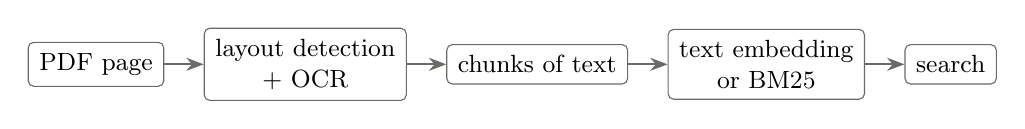
\begin{tikzpicture}[node distance=5mm]
  \node[box] (p) {PDF page};
  \node[box, right=of p] (o) {layout detection\\+ OCR};
  \node[box, right=of o] (c) {chunks of text};
  \node[box, right=of c] (e) {text embedding\\or BM25};
  \node[box, right=of e] (s) {search};
  \draw[arr] (p) -- (o); \draw[arr] (o) -- (c); \draw[arr] (c) -- (e); \draw[arr] (e) -- (s);
\end{tikzpicture}\\[10pt]
\begin{itemize}
  \item slow to build (OCR, captioning), and it breaks easily;
  \item tables, charts, logos and layout are lost or garbled;
  \item OCR errors become search errors.
\end{itemize}
\vspace{4pt}
\textcolor{muted}{Two modalities meet here: the document is an \emph{image}, the question is \emph{text}.}
\end{frame}

% ------------------------------------------------------------------------------------------------------
\begin{frame}{ColPali: search the page \emph{image} directly}
\begin{columns}[T]
\column{0.58\linewidth}
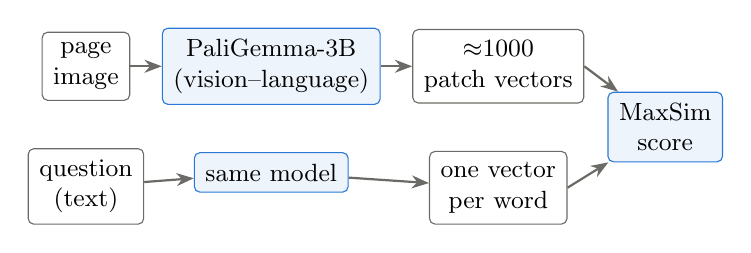
\begin{tikzpicture}[node distance=4mm, every node/.append style={font=\scriptsize}]
  \node[box] (img) {page\\image};
  \node[hot, right=of img] (vlm) {PaliGemma-3B\\(vision--language)};
  \node[box, right=of vlm] (pv) {$\approx$1000\\patch vectors};
  \node[box, below=6mm of img] (q) {question\\(text)};
  \node[hot, below=6mm of vlm] (lm) {same model};
  \node[box, below=6mm of pv] (qv) {one vector\\per word};
  \node[hot, anchor=west] (ms) at ($(pv.east)!0.5!(qv.east)+(4mm,0)$) {MaxSim\\score};
  \draw[arr] (img) -- (vlm); \draw[arr] (vlm) -- (pv);
  \draw[arr] (q) -- (lm); \draw[arr] (lm) -- (qv);
  \draw[arr] (pv.east) -- (ms); \draw[arr] (qv.east) -- (ms);
\end{tikzpicture}\\[10pt]
\small $\text{score}(q,d)=\sum_{\text{words } i}\ \max_{\text{patches } j}\ \langle q_i, d_j\rangle$\\[3pt]
\textcolor{muted}{\footnotesize each question word finds the patch where it ``appears'' on the page - no OCR}
\column{0.39\linewidth}
\begin{itemize}
  \item Faysse et al., \emph{ColPali}, ICLR 2025.
  \item Same scoring idea as ColBERT (text search), applied to image patches.
  \item \Pub{} On the ViDoRe benchmark it beats every OCR-based pipeline: average nDCG@5 \textbf{81.3} vs \textbf{67.0}.
  \item New model family since then: ColQwen, Tomoro, \dots
\end{itemize}
\end{columns}
\end{frame}

% ------------------------------------------------------------------------------------------------------
\begin{frame}{My question: does keyword search still add anything?}
\begin{itemize}
  \item In \emph{text} search, combining \textbf{keyword search (BM25)} with \textbf{semantic search} is a cheap, standard improvement (``hybrid search'').
  \item Visual retrievers might miss exact strings: invoice numbers, codes, names.
  \item \textbf{Question:} if we add BM25 over the page's OCR text to ColPali, does page retrieval improve? For which questions?
\end{itemize}
\vspace{6pt}
\textbf{What I did}
\begin{enumerate}
  \item Reproduced ColPali on ViDoRe DocVQA with the authors' code and checkpoint.
  \item Fused it with BM25 using reciprocal rank fusion, plus a \emph{control} (a dense text model instead of BM25).
  \item Fixed predictions and settings in advance; tuned on a dev split; touched the test split once; significance tests.
  \item Follow-ups: stronger text pipelines, newer Qwen models, and the same test on the nine other ViDoRe tasks: infographics, arXiv figures, French tables, financial reports, and topic collections (energy, government, healthcare, AI, French environmental reports).
\end{enumerate}
\end{frame}

% ------------------------------------------------------------------------------------------------------
\begin{frame}{What came out}
\centering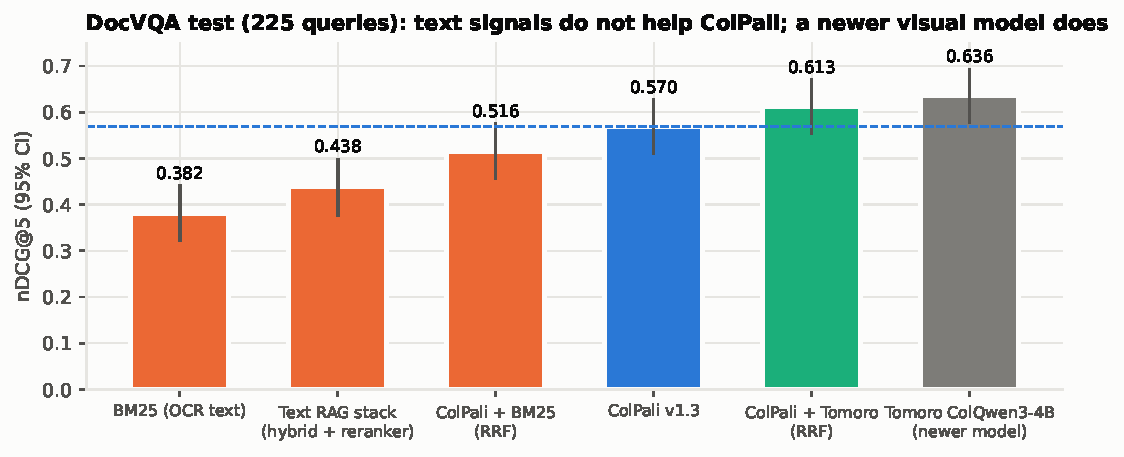
\includegraphics[width=0.8\linewidth]{fig9_talk_summary.pdf}\\[2pt]
\raggedright\small
\begin{itemize}
  \item \Mea{} The reproduction holds: nDCG@5 \fullB{} vs \pubCard{} reported by the authors.
  \item \Mea{} Adding text never helped: BM25 fusion \deltaC{} on DocVQA, and no significant gain on any of nine more ViDoRe tasks.
  \item \Mea{} A newer \emph{visual} model did: Tomoro ColQwen3-4B \deltaTM{} here, \infoDelta{} on a task never used for tuning.
\end{itemize}
\end{frame}

% ------------------------------------------------------------------------------------------------------
\begin{frame}{Take-aways for your own projects}
\begin{itemize}
  \item \Int{} \textbf{Visual document retrievers already ``read'' the text.} OCR-based keyword search mostly finds pages ColPali finds anyway.
  \item \Int{} \textbf{Fusion is not free.} Combining two rankers helps when both are comparably strong; a much weaker one imports its errors. This matches findings in text retrieval (Bruch et al., TOIS 2024).
  \item \textbf{Method matters as much as the score:} a control system, a held-out test set used once, and a fresh task for confirmation turned a ``negative'' result into a clear answer.
\end{itemize}
\vspace{10pt}
\begin{block}{More detail}
\small Report, code, all results and the detailed slides:\\
\texttt{github.com/ismailucrn/colpali-hybrid-retrieval} \quad(tag \texttt{v1.0-submission})
\end{block}
\end{frame}

\end{document}
